\section{Mozart/Oz}

Mozart is an implementation of the multiparadigmatic language Oz. Oz is a functional
language with built-in support for threaded applications and paralelisation. It also
contains support for constraint solving. It also supported to run subroutines on computers
connected to the cluster. Since it is a multi-paradigmatic language the user
can write imperative as well as Prolog-like programs. The language also offers classes
including inheritance and creating the objects. The language was designed for the
highest variability of usage because the programmer can use all the features of imperative,
functional, logic, object-oriented and other paradigms in one program. In the standard distribution
it is shipped as a standalone compiler which compiles into native executable code.
Moreover it can run in the interactive mode. The programmer can feed the compiler with
a single line, buffer or whole program and the compiler immediately responds. As an IDE
Mozart standardly uses EMACS system.

Just like in any other functional language the programmer can assign to the variable 
only once per its lifetime. Therefore all variables holds also its state. In case that
an operation is performed over the not assigned variable the actual command is suspended
until the problem is resolved. This means that after executing the following code the
variable $c$ will contain 5:

\begin{verbatim}
a = 5
if a > b then c = 5 else c = 6
b = 4
\end{verbatim}

\subsection{Solver description}
As stated in the previous section the language has integrated a constraint solver. The solver
can solve problems with variables whose domains are finite sets. A finite domain
set can contain the natural numbers including zero. The maximal value of variable is limited and is smaller 
than the maximal integer. The computation model for constraint propagation is called 
a Space. The space consists of several propagators connected to a constraint store.
The constraint store contains conjunction of ground constraints. Ground constraints
are constraints in the form $x=n$ or $x \in D$. For example the constraint store could
contain the constraint $x = 6 \mand y \in \{1, ..., 12\} \mand z = y$. Propagators contain
other constraints, for example $x>y$ or $a^2 + b^2 = c^2$. Propagator for a constraint
 $c$ is an independent agent who tries to shrink the domain of variables constrained
 by $c$. A solution is such  anassignment of values to variables which satisfies all the conditions
 in propagators.
 
\begin{example} Let us have variables $X$ and $Y$ and the following constraints: $X \in \{0..9\}$, $Y \in \{0..9\}$, 
  $X+Y = 9$, $2X + 4Y = 24$. 
\begin{enumerate}
  \item The constraint store contains: $X \in \{0..9\}$, $Y \in \{0..9\}$. Propagators: $X+Y = 9$ a $2X + 4Y = 24$.
  \item	The first propagator cannot do anything but the second changes the constraint store to $X \in \{0..8\}, Y \in \{2..6\}$.
  \item	The first propagator changes the constraint store to $X \in \{3..7\}$, $Y \in \{2..6\}$.
  \item	The second propagator changes the constraint strore to $X \in \{4..6\}$, $Y \in 3..4$.
  \item	The sirst propagator changes the constraint store to $X \in \{5..6\}$, $Y \in \{3..4\}$
  \item	The second propagator finally changes the constraint store to $X = 6$, $Y = 3$.
\end{enumerate}
\end{example}

Propagation can be either interval or domain. The interval propagation changes only 
the bounds of domain. Domain propagation also eliminates the values of the domain.
The domain propagation is on the first sight better technique but is more complex
than the interval propagation. Therefore the interval propagation is more frequently used.

After propagation if the system is in a stable state and still the solution was not found
the distribution phase begins. Mozart choose a variable $x$ and value $v$ from domain
 $D_v$ and create two new spaces $S \cup \{x = v\}$ and $S \cup \{x \neq v\}$.
 The computation then continues with the propagation phase in the new spaces.
 If the propagation phase ends with a failure the space also fails. The problem has no
 solution if all its spaces have failed.

We can choose from several distribution strategies. Choosing of the proper strategy 
noticable affects the computation time.  For most problems the first-fail strategy is
the most suitable. However the user can implement his own distribution strategies to fully
suit his needs.

Two techniques can be used in the solving of the optimalisation problems. The na\"{i}ve 
technique introduces auxiliary variable $o$ and adds the constraint $o = f(P)$ where $f$ is the
objective function. Then the variable $o$ is increased until the the solution is found. The second possible
technique is the branch-and-bound algorithm which is described in the section \ref{introduction:constraint-programming}.

\subsection{Debugging support}
Mozart/Oz offers to the user the interactive tool Explorer. The Explorer can be used to explore 
the search tree including the choice nodes. The user can use the Explorer in the 
interactive mode and choose the subtrees of the search tree to be expanded. 
 The Explorer tool screenshot is in the figure \ref{mozart:explorer}. The circles 
 denotes the choice nodes of the tree, the diamonds means the solution of
 the problem and finally the squares are the branches with no solution. The lighter color
 denotes the nodes which can be expanded. On the figure there is one solution, two 
 unsuccesful branches and five choice nodes. Three of the choice nodes can be still expanded.
 The Explorer tool offers also exporting off the tree diagram to PostScript.

\begin{figure}
\caption{\label{mozart:explorer}The Explorer tool}
\begin{center}
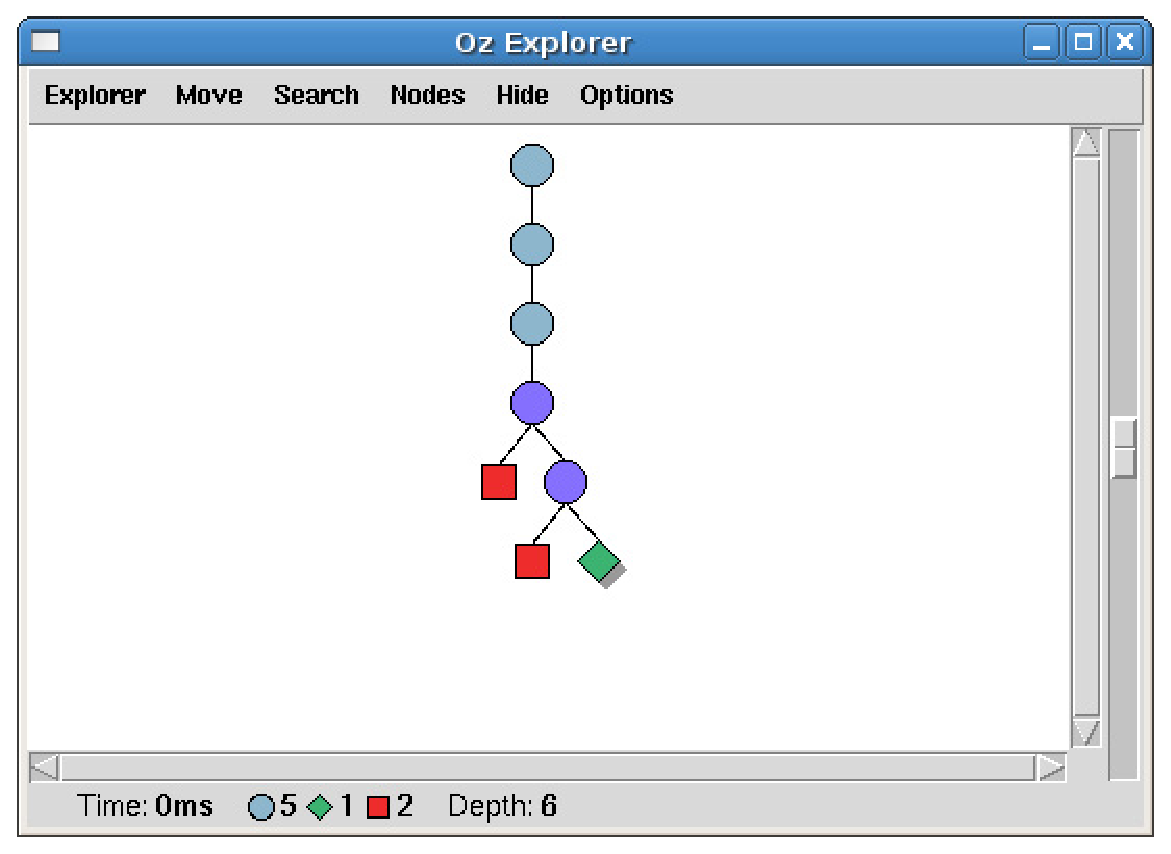
\includegraphics[scale=0.3]{images/screenshoty/explorer.eps}
\end{center}
\end{figure}


\subsection{Subjective description}
The Mozart/Oz system is well documented. There is available a website \cite{mozart:documentation} where the reader
can find the documentation for the whole system. The difficulty level of the documentation
varies from the tutorials and basic documentation to the advanced topics. The Oz language 
was new for the author of this thesis but the documentation was sufficient 
to understand the programs written in Oz and to be able to write new programs by
himself. The development of the system seems stopped. The last version was released
a year ago. The release contained a bug which results in a problems while the compiling
of the Mozart. There has been nothing done about it even though the authors statement
that the bug will be corrected.